\chapter{Research}

I propose a framework to examine remixing in an online community of amateur creators. 
I approach this by first studying the design of the online community as a remixing system, and then analyzing what people do and how they react to what others do.
More specifically, I focus on the structural, functional and attitudinal characteristics of an online community's sociotechnical infrastructure and its participants activities.
This framework derives from and is examined through design interventions, three-years of participant observation data, case studies, interviews with community members, quantitative and network analysis of a large corpus of data that includes more than 700,000 registered accounts and a repository of more than 9 million comments and 1.6 million interactive media objects, 30\% of which are remixes.

\section{Structure of a Remixing System} 
I plan to study the sociotechnical architecture of the Scratch Online Community by examining its following structural attributes (Figure~\ref{fig:structure}):
1) granularity of the remixable components, 
2) modularity of the remixable components, 
3) decomposability of finished projects, 
4) attributability mechanisms and 
5) openness to remix across systems.

In this proposal I briefly define each structural attribute using one or two examples and I explain how I am planning to go about studying it.
I plan to do analyze these structural properties of the system using varied approaches including:
1) case studies that give an rich description of different scenarios that elucidate on the influence of each attribute,
2) analyses the data corpus to understand the frequency of the scenarios and the relationships between the structural attributes,
3) natural design experiments to study the effect of varying some of the structural dimensions.

\begin{figure} 
\centering
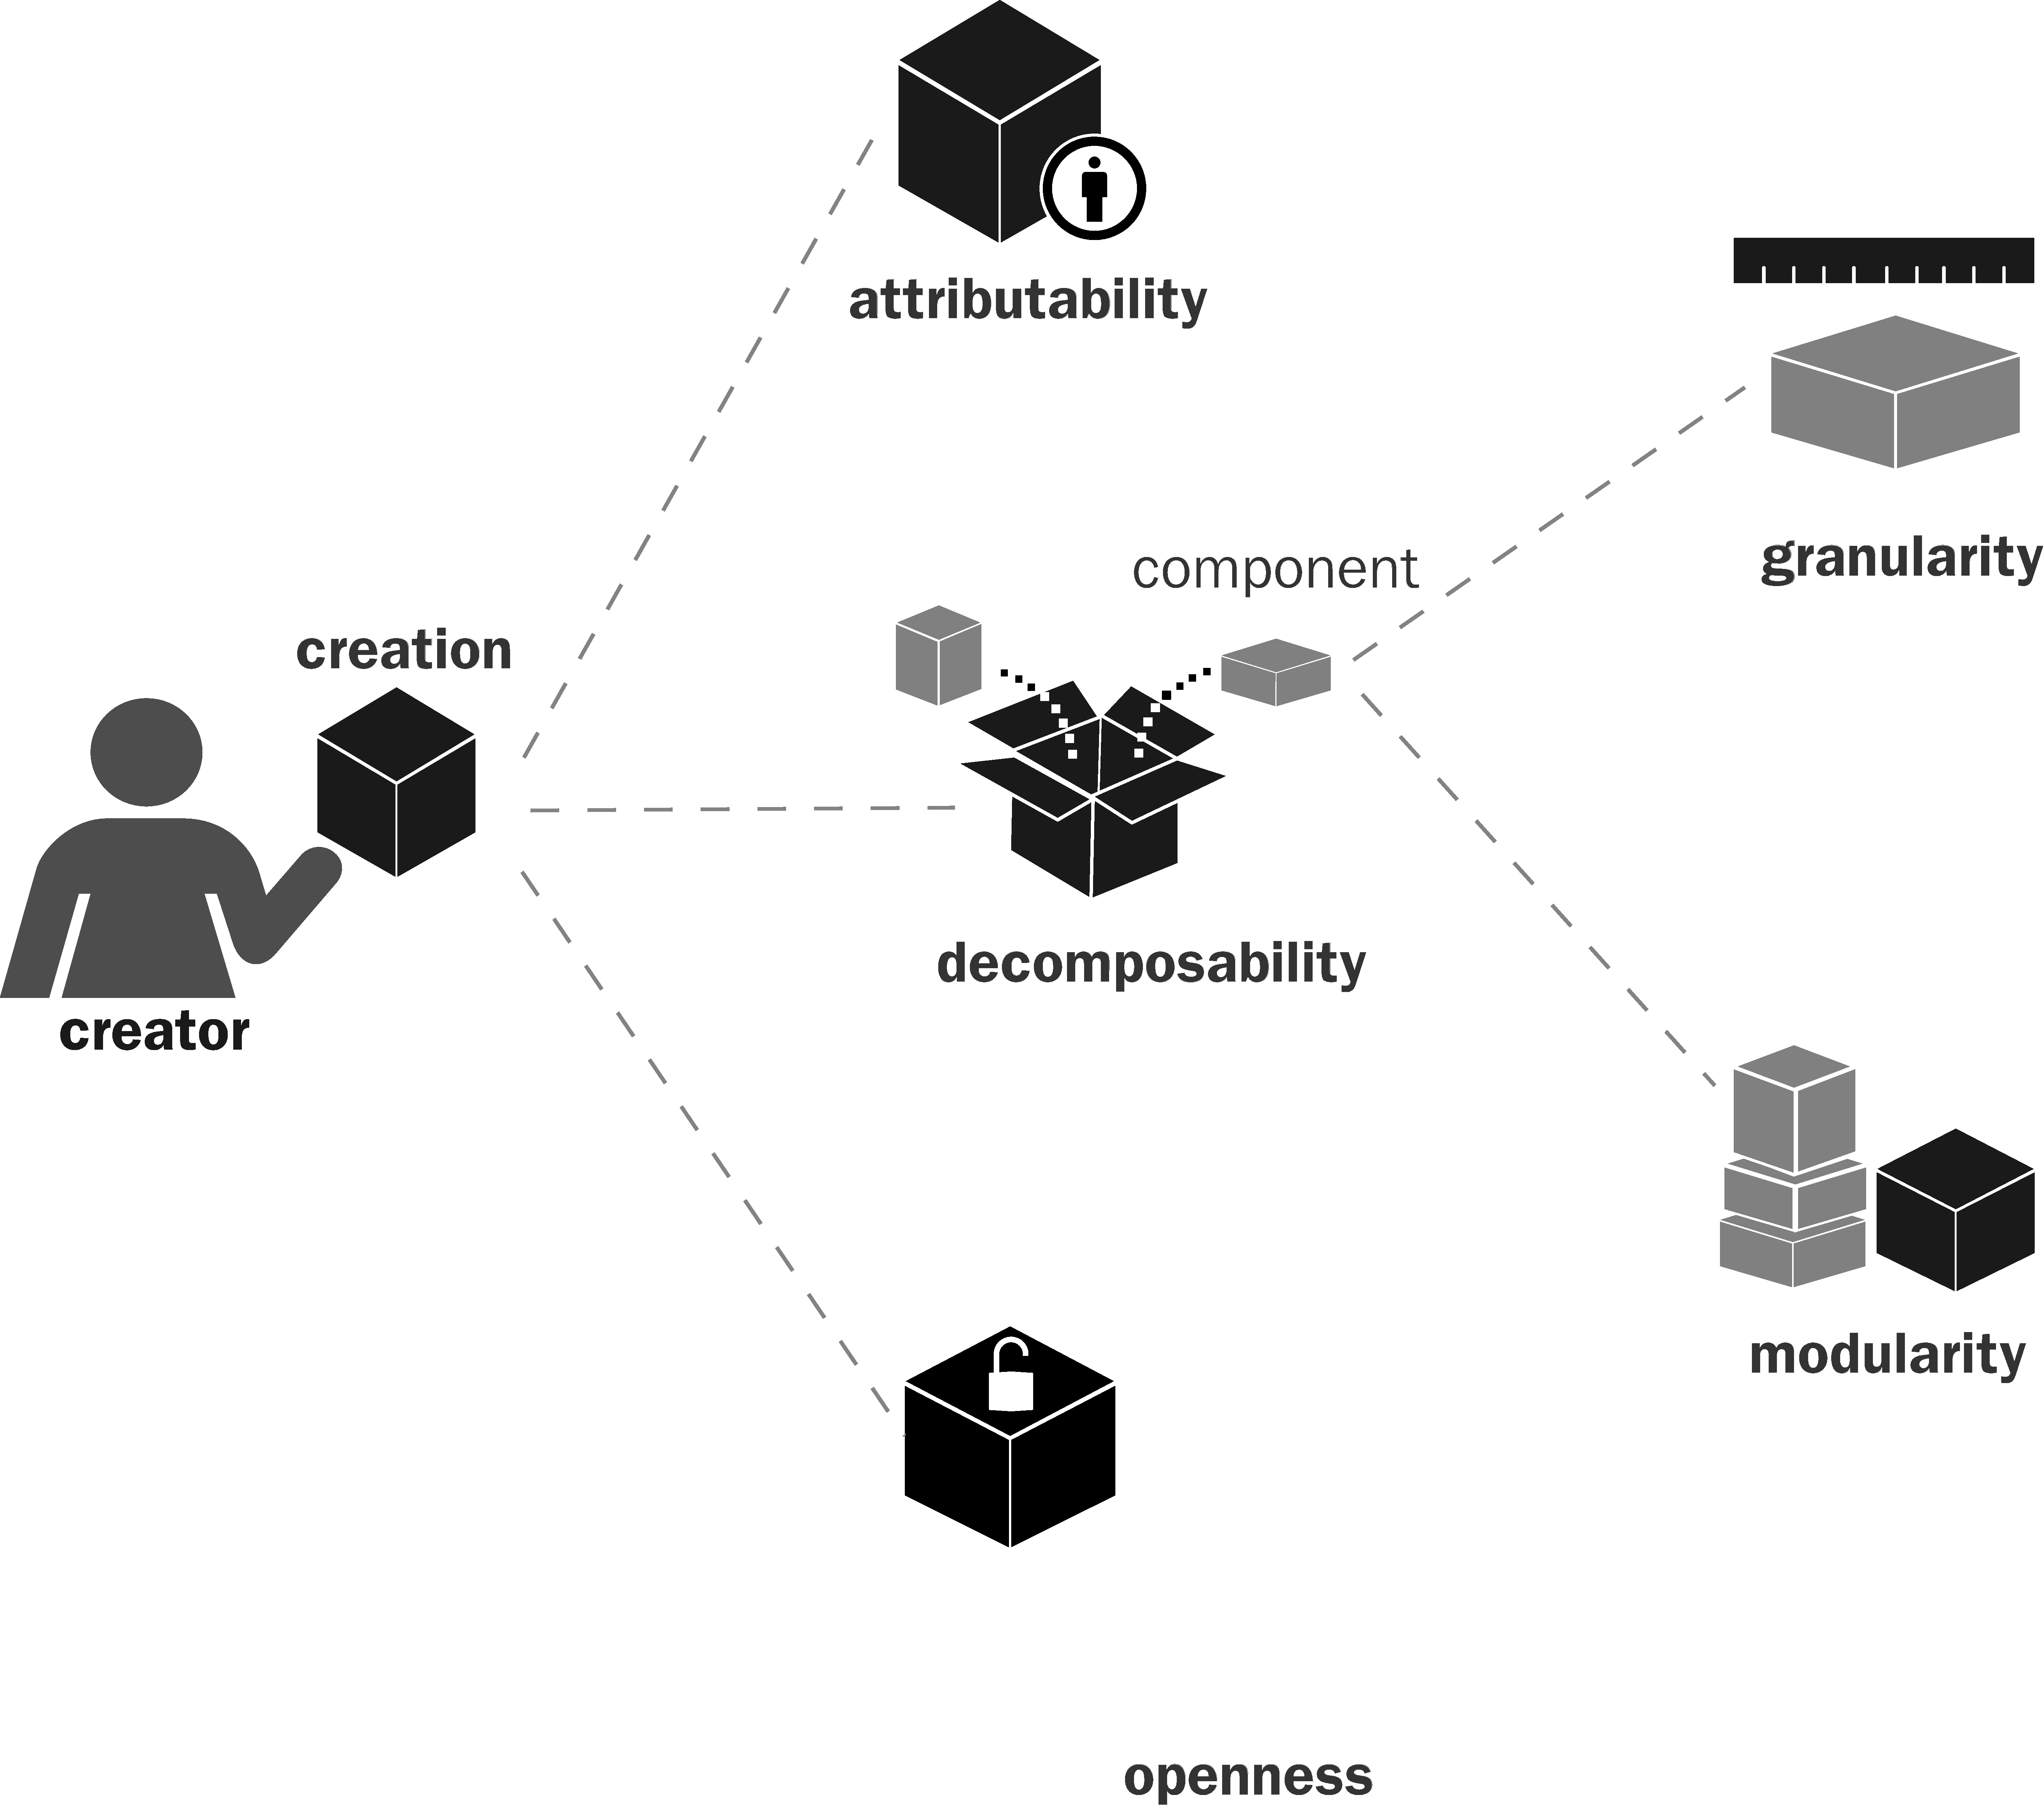
\includegraphics[width=3.25in]{figures/structure.pdf}
\caption{Structural dimensions of a remixing system}
\label{fig:structure}
\end{figure}

\subsection{Granularity}
Granularity is the size of projects' modules \citet{benkler_coases_2002}. 
In Scratch, projects have a couple levels of granularity.
Projects are made up of ``sprites'', for example, characters in a game or a elements in the user interface elements of an interact simulations.
Each sprite can have ``scripts'' or  stacks of programming blocks that control the sprite's behavior such as its position on the screen, its looks, sounds and interaction with other sprites and the user (via mouse, keyboard, or other sensors).
Each sprite also has one or more costumes or images that represent the different visual states of a sprite.
Sprites can also have sounds that are played programmatically, for example, a character in a game could make a sound each time it jumps.

\subsubsection{Proposed work}
The Scratch Online Community, by default it only allows for sharing at the coarsest degree of granularity: only projects can be shared. 
I plan to analyze the implications of this design decision and the ways  people get around the limitations of the architecture.

I have anectdotal evidence that Scratch participants get around the granularity limitations by sharing full projects with the sole intention of sharing a single sprite, script, image or sound.
This need for finer granularity often stems from a desire to engage in sharing practices that the original design did not anticipate. For example, I have documented before the existence of ``coloring contests'' \citep{nickerson_appropriation_2011} where Scratch community remix in order to add color to an image. or as part of group collaboration.
I plan to look these practices in more detail to understand the ways in which a finer granularity mechanisms would help support different types of creative and collaborative learning practices beyond the the existing research that suggests that finer granularity is correlated to the number of people engaged in cooperative activities.

In order to analyze the effect of explicitly supporting finer degree of granularity through a natural experiment, I plan to analyze the adoption ``Scratch Resources'' \footnote{Available at http://resources.scratchr.org}, a website created by members of the Scratch community to support sharing sprites, images and sounds. 
% TODO link to Von Hippel at al on user innovation

Some of my motivating questions are: 
how common is sharing and remixing across the different levels of granularity available (even if not explicitly supported)?
what are the types of participants and motivations for sharing finer grained components?
what role does granularity play in the likelihood of a project being remixed controlling for all other factors?
how do different levels of granularity impact the type and quality of remixes?
how do different levels of granularuty support different levels of familiarity with Scratch, that is, are novices more likely to rely on coarser granularity when engaging in remixing as a scaffolding mechanism?

\subsection{Modularity}
\citet{benkler_coases_2002} defines modularity as the ``property of a project referring to the extent to which it can be broken down into smaller components, or modules, that can be independently and asynchronously produced before they are assembled into a whole.''
For the purpose of this work, I will separate two different aspects of modularity:
1. The ease of \emph{integrating} such components into new creations or remixes.
2. The ease of \emph{decomposing} an existing project into smaller components, typically for the purpose of remixing.
In this section I plan to analyze the term ``modularity'' by focusing on the first aspect.
In the next section, I will focuson the second aspect under the term ``decomposability''.

\subsubsection{Proposed Work}
There are some components or projects that can be more easily integrated into new projects. 
One of the questions I am intersted in exploring is what makes some components more modular than others.

For example, an image generated programmatically might be harder to integrate than one in bitmap format. 
A module that representing a cultural icon, such as Mario\footnote{Mario is a character in a popular video game called Mario Bros. from Nintendo Inc.}, is perhaps easier to integrate into other projects than an image of a less well-known character.
However, there are situation when new subcultural icons emerge within the Scratch community.
For example, a character called Maki-Tak created by a community member from New Zealand started a whole genre of projects, called Takis.
These projects use adaptations of that lizard. 
% Other examples: Mr happy Man
There are also situations where some components are remixed despite their internal complexity which might indicate that these could be built in a way that their internal complexity is hidden and remixing them is easy. 
For example there is a sprite created by an advanced Scratch user that represented a physics simulation of a string. 
This project was later remixed in a project where it represented a necklace.

I plan to operationalize the assessment of modularity by measuring its adoption through number of remixes.
The assumption will be that more modular components are remixed more.
I will examine this in two types of components:  ``samples'' and ``community-generated''.
% Sample components are those that come pre-installed with Scratch. For example, sample images, sounds, sprites and projects in some cases.
% Community-generated are those created by end-users.
For example, ``jetpack girl'' is a sample script consisting of five costumes and  sounds for a flying character that can be controlled with the keyboard.
The code of the sprite comes with an invitation to remix: ``Import me into your own project'' and an explanation on how to use it ``arrow keys make me fly''.
These sample components are not only sprites, there are also hundreds of images and sounds that come with Scratch such as photos of people, animals, things, etc.
In addition to these sample components, there are thousands of components created by community members that are remixed and that can be found in places like Scratch Resources and Scratch projects that explicitly state that they include sprites, images and sounds for others to reuse.

The type of questions I will try to answer are then are:
1. What technical or cultural attributes are linked with component modularity? 
2. Are more modular components used more often by newcomers and do they provide scaffolding in their learning of Scratch programming?
3. Are community-generated components more often created by advanced users?

\subsection{Decomposability}
Building on the concept of modularity examined before, in this section I will examine decomposability as the ease of decomposing a compiled project.
Decomposability is the ease of breaking something apart for the purpose of remixing it.
Therefore decomposability depends on the internal complexity of a project, which in itself is dependent on the expertise of the person attempting to decompose the project.
For example, one can argue that images in Flickr.com are harder to decompose than those in OpenClipart.org, which provides the source vectors, or Aviary.com which provides the bitmap images that were used to create an image.
The same happens with software applications that provide the source code in contrast with thost that only provide the final compiled executable.
But even if the source is provided, there are some cases where projects are ``impenetrable'' due to their complexity or a missmatch between the expertise of the person trying to decompose a project and the complexity of the project. 
For example, for a novice programmer having access to the source code of the Linux kernel might not allow for easy decomposability.

In Scratch, all the sources of a project are provided so the decomposablity of a project depends, among other things, more on how interconnected its different components are. 
For example, sometimes sprites ``broadcast'' messages back and forth making their decomposablity much harder than those that are self-contained.
Also, some creators add instructions to their projects explaining how they can be broken apart, while others obfuscate their code to prevent remixing.

\subsubsection{Proposed Work}
I will first do a manual analysis of a sample projects to observe patterns of decomposability. 
Using the findings of this analysis I will come up with mechanisms to automate the evaluation of decomposability. 
For example, it is possible that a decomposability metric could depend on the use of particular blocks (the ``broadcast'' block could reduce its ranking, while comments in the code would increase it), explicit obfuscation or matching between the average expertise level of community members and the expertise required to understand a project.

I will also look at remixes to analyze how different they are from their original project. 
The assumption would be that ``impenetrable'' projects would be correlated with no remixing or to superficial remixes, such as slights changes in the images,
while highly decomposable projects are associated with significant differences betweent the remix and the original.

I will also analyze in detail the practices of code obfuscation and the strategies people use to discourage decomposability of their projects.

\subsection{Attributability}
Creators often want to get credit for their work. 
For example, the Creative Commons license originally had attribution as one of the options of their licenses but after analyzing several years of usage of the licenses they found that very few people waived the attribution clause. 
This led them to include attribution by default in all their licenses (and create a separate license for completely public domain works) \citep{brown_announcing_2004}
In order to further our understanding of attribution when desigining a remixing system it is important to know the role attribution plays in supporting cooperative behavior among members of a remxing online community.

In Scratch, we have run some design experiments playing with attribution. 
For example, we found evidence that suggests that about 20\% of creators object to seeing their projects remixed \citep{hill_responses_2010}.
We also have anectdotal evidence that people who objected to remixing of their project referred to lack of credit as one of the problems.
In order to address this,I added a mechanism that would automatically give credit to the creator of the original project whenever a remix was uploaded (e.g. ``Shared by John, based on Mary's project'').
Using that design intervention as a natural experiment, we found evidence that suggests that people not only want to get credit but that they prefer the credit given by another person over the automatic attribution given by the system \cite{monroy-hernandez_computers_2011}. 

\subsubsection{Proposed Work}
I plan to extend this work with additional experiments.
For example, one of the common complains against remixing is that the textual description of projects often gets copied from an original project onto its remixes.
This often gives the wrong impression that those notes were written by the remixer rather than the original creator.
I plan to add a mechanism to show a distinction between the notes written by the originator and those added by the remixer.
These additional notes will come with a mechanism to encourage remixers to explain the ways in which the original project was changed.
This will serve as a natural experiment to test out the additional value of not only giving binary representation of attribution but also give a qualifier explanation to the connection between a remix and the original project.

% TODO: Other experiments: 
% - Creator endorsed attribution.
% - Diff

\subsection{Openness}
Openness is not onl
% Across systems. Ethos explained. Creative commons version for kids. DeviatnArt conflicts
% 



I analyze the role remixing plays in participating in an online community of creators.
I look at how several forms of remixing (Figure~\ref{fig:function} are represented in the Scratch Online Community, how their use evolves, and how they do or do not support sociability and creative practices.
I analyze people's remixing behavior including their: 
1) modifying existing work, 
2) reusing components, 
3) collaborating with others in groups, 
4) persuading crowds to join remixing chains, 
5) inspiring others with ideas for new creations or 
6) self-appropriating their work to create something. 

\begin{figure}
\centering
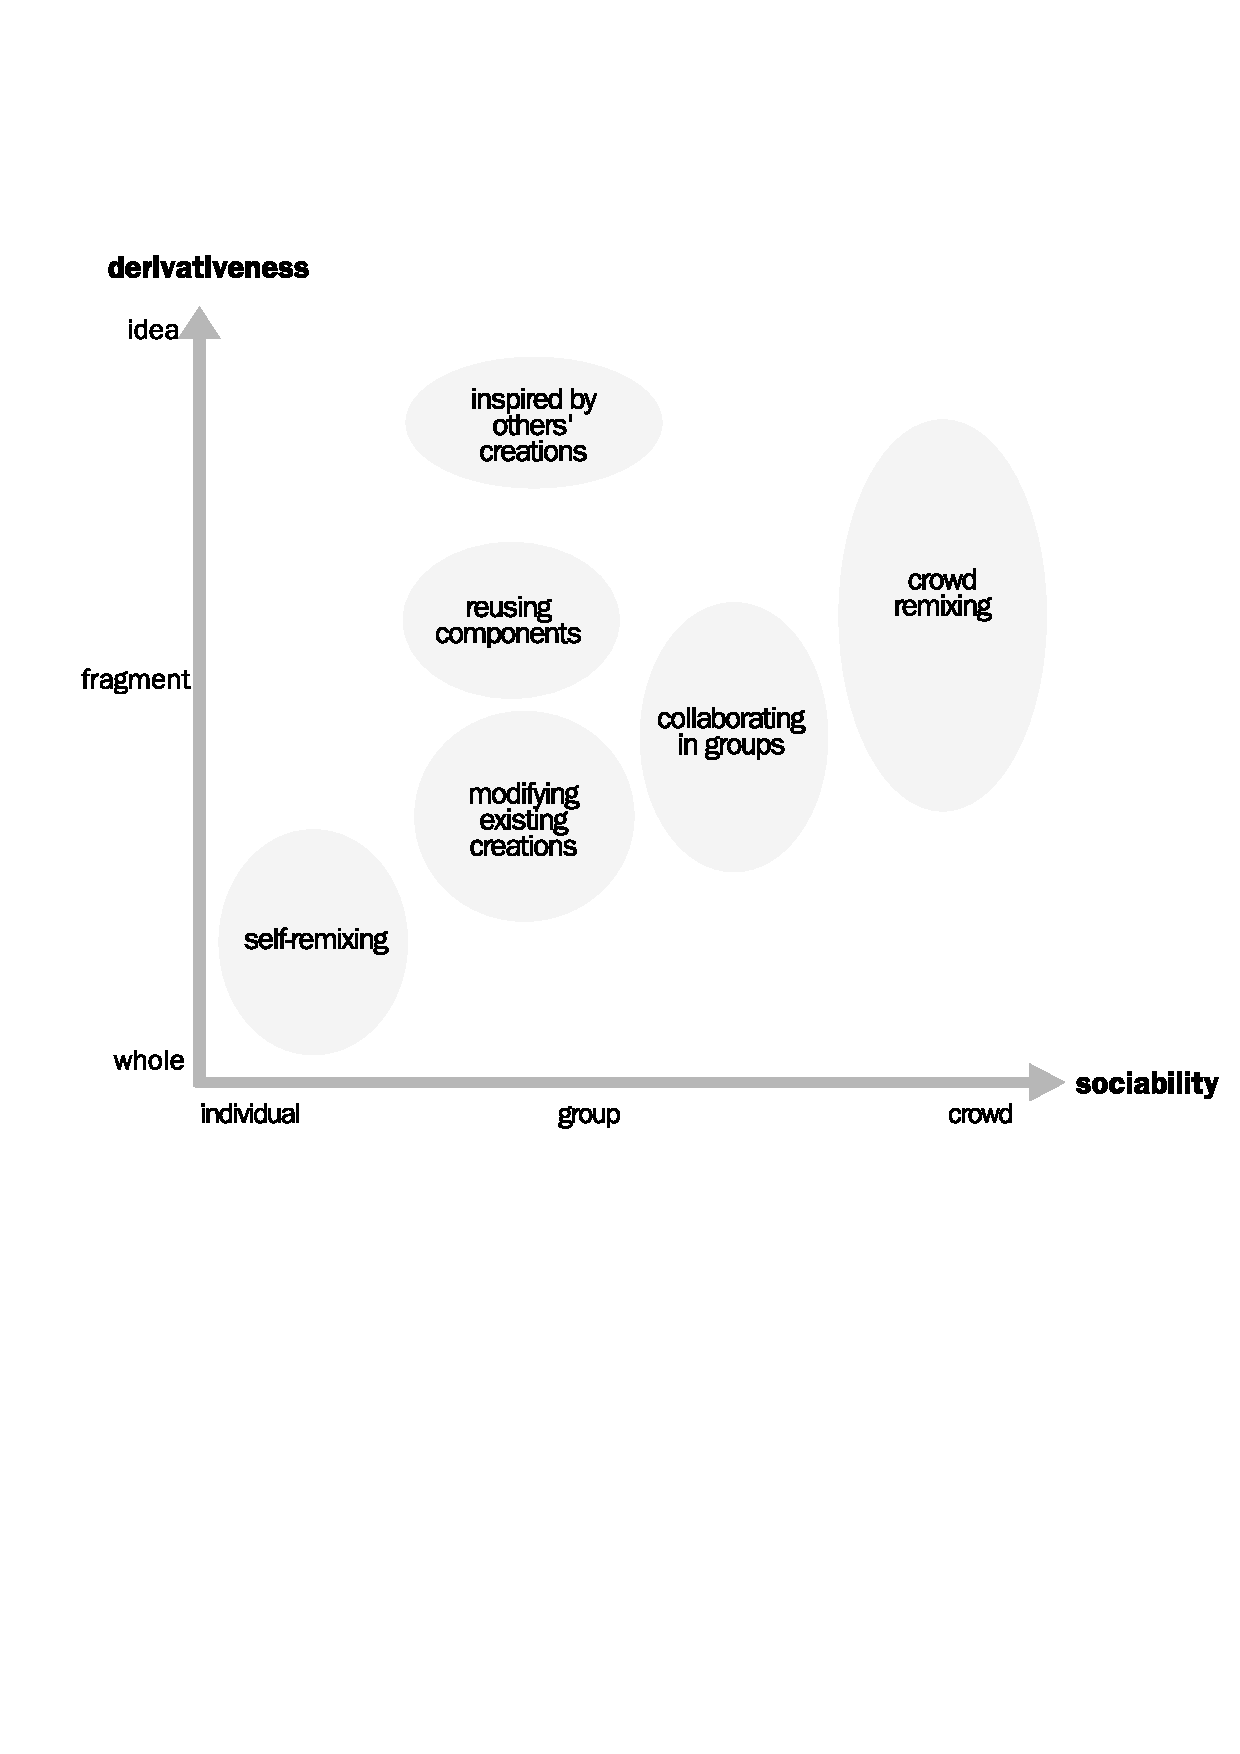
\includegraphics[width=3.25in]{figures/function.pdf}
\caption{Functional roles of remixing in the social and produc-focus dimensions}
\label{fig:function}
\end{figure}

% TODO:
% Proposed work:
% - Evolution of each type.
% - How do they engage in these different forms of production.
% - To what extent do these different forms of remixing support:
% a) scaffolding,  b) committment, c) creative and d) collaborative practices? e) reputation
% 	Look at people who get started by remixing and compare it to those who don't. Follow take other pats.
% 1. Modifying existing work. 
% 4. Crowds: coloring contests
% Some of these roles are analyzed from a network perspective. For example, the network of people engaged in colloring contests represents a group of people involved in a gift exchange network.


\subsection{Attitudes Toward Remixing}

I investigate remixers' and originators' attitudes toward remixing. In particular, I analyze how participants perceive remixing and how they do or do not cooperate by letting or encouraging others to reuse their work.
This analysis is driven by an interest in understanding how the system design may influence these attitudes. 
I plan to analyze these issues from the perspective of people whose projects are remixed as well as from those creating the remixes.
 
Previous work studying people's attitudes toward remixing in the Scratch Online Community \citep{hill_responses_2010, monroy-hernandez_computers_2011} found evidence that people are as likely to react negatively as they are to react positively when someone remixes their work. 
Additionally, we have found originators are more likely to respond negatively when their projects are more complex.

Broadly speaking, people whose projects are remixed react either by being indifferent to it, accepting it, conditionally accepting it (for example, specific rules or norms have to be followed), or by explicitly opposing to it (for example, posting a negative reaction comment like ``you stole my project!'').
Similarly, remixers go about remixing by either being oblivious of the norms (for example, giving credit or asking for permission has emerged as a norm in the  community), or cautiously doing it by asking for permission first, or even being confrontational and using remixing as a form of ``trolling'' \citep{donath_identity_1998}.

\subsubsection{Proposed Work}

I plan to analyze people's attitudes toward remixing in the Scratch Online Community through case studies and experiments.
Additionally, I expect these metrics of people's responses and attitudes will serve to understand the health of the community and to motivate further design interventions.
In particular, I propose two studies for studying Scratch participant's attitudes toward remixing that complement the two recently published articles \citep{monroy-hernandez_computers_2011,hill_responses_2010}.


% NOTES The overarching questions are: How do young people respond to remixing? How are these attitudes represented in the community? When do they embrace remixing and when do they reject it?  I have and will analyze young people’s attitudes based on their words (interviews) comments, reports (flags) and strategies for deterring (obfuscation, pseudo-licenses, Vigilantism) or supporting remixing (commenting, scaffolding, framework approach, creation of narratives).
% Crowding out remixing by featuring
% Evolution of reactions as design changes

\emph{Plasticity of Virtue.}
For the past five months, I have been running an experiment aimed at ascertaining how people's attitudes toward remixing could be changed through a design intervention.
The study consists of sending notification messages that try to appeal to various motivations for cooperating in the Scratch online community. 
As mentioned before, a contentious issue in the Scratch community has been the acceptance of remixing by those whose projects are remixed. 
People only learn about remixes of their projects by browsing their project pages and looking at the list of derivative works. 
The notification page is the principal form of communication between the system and the users.
The experiment consists of informing people when one of their projects gets remixed.
This experiment provides an opportunity to test: 1) the comparative effectiveness of various ways of communicating the same event and 2) the permanency of the behavioral change, if any. 

The experiment consists of two phases.
The first is the notification period. 
When someone's project gets remixed, the system automatically assigns the creator of that project to one of the treatment conditions. 
From then on, the person receives messages whenever someone remixes his or her project. The message depends on the treatment category.
For example some messages are neutral (for example, ``Your project FooBar was remixed. Check out the remix.''); 
others are positive (for example,``Congratulations! Your project FooBar was remixed. Check out the remix .'');
others try to elicit generosity (for example, ``Your project FooBar has been remixed. Sharing your work is a generous thing to do and a great thing for the Scratch community! Check out the remix.'').
Other messages try to elicit conformity, reputation building and fairness.
Finally, a control category is added where no notification is sent.

The second phase of the experiment is sending no notifications. In this phase of the experiment, the notifications stop and people's reactions continue to be logged.

After a few weeks we look at the results of pre- and post-phase one, to analyze the effectiveness of each treatment by measuring the number of positive and negative reactions that originators leave on the remixes. 
Additionally, I analyze the pre- and post-phase two, to see how malleable the behavior is.

\emph{Featuring Top Remixes.}
The home page of the Scratch website now has a section called ``What the Community is Remixing''  that features the three top remixed projects in the past two weeks.
This section did not exist when the website was first unveiled.
In fact, this section was added as measure to counter the backlash against remixing by showing that getting one's project remixed could increase social status in the community (being on the front page is an important reputation-building mechanism).
This study aims at assessing whether a design intervention aimed at increasing the acceptance of remixing had a ``crowding out'' effect by decreasing the quality or effort people put into making their remixes.
I have devised metrics to operationalize the complexity and effort a creator puts into creating his or her project. These metrics are based on the number of sprites, scripts, blocks, diversity of blocks and time it took from the first save to the hard disk until it gets shared on the website.



